\documentclass[11pt,a4paper]{article}
\usepackage[margin=2.5cm]{geometry}
\usepackage{booktabs}
\usepackage{longtable}
\usepackage{array}
\usepackage{hyperref}
\usepackage{xcolor}
\usepackage{enumitem}
\usepackage{parskip}
\usepackage{fancyhdr}
\usepackage{microtype}
\usepackage{tikz}
\usetikzlibrary{shapes.geometric, arrows.meta, positioning, fit, backgrounds}

\hypersetup{
    colorlinks=true,
    linkcolor=blue!70!black,
    urlcolor=blue!70!black,
    citecolor=blue!70!black,
}

\pagestyle{fancy}
\fancyhf{}
\rhead{KRAKEN Bug Reports}
\lhead{SRSE 2026 -- Mahadi Hasan}
\rfoot{\thepage}

\title{\textbf{Bug Reports for the paper:\\
\textit{KRAKEN: Program-Adaptive Parallel Fuzzing}}}
\author{Mahadi Hasan \\ \small UIUC SRSE 2026}
\date{\today}

\begin{document}
\maketitle
\thispagestyle{fancy}


\tableofcontents
\newpage

%----------------------------------------------------------------------
\section{Introduction}

\textit{KRAKEN: Program-Adaptive Parallel Fuzzing} (ISSTA 2025,
\url{https://dl.acm.org/doi/10.1145/3728882}), presents a new program-adaptive parallel
fuzzer. As part of evaluating KRAKEN's effectiveness, the authors ran it against 37
popular open-source projects and reported the following results:
\begin{itemize}[nosep]
    \item \textbf{192 bugs} found across 37 real-world projects
    \item \textbf{119 CVE IDs} assigned to those bugs
\end{itemize}
These bugs were reported to the developers of the affected software, typically as GitHub
issues or pull requests (but also via Bugzilla, SourceForge, and mailing lists).

%----------------------------------------------------------------------
\section{Search Process}

The overall strategy is illustrated in Figure~\ref{fig:flowchart}. The process splits into
two paths after extracting the CVE list: a CVE-based automated path and a manual path for
the six projects with no CVE assignments.

\begin{figure}[htbp]
\centering
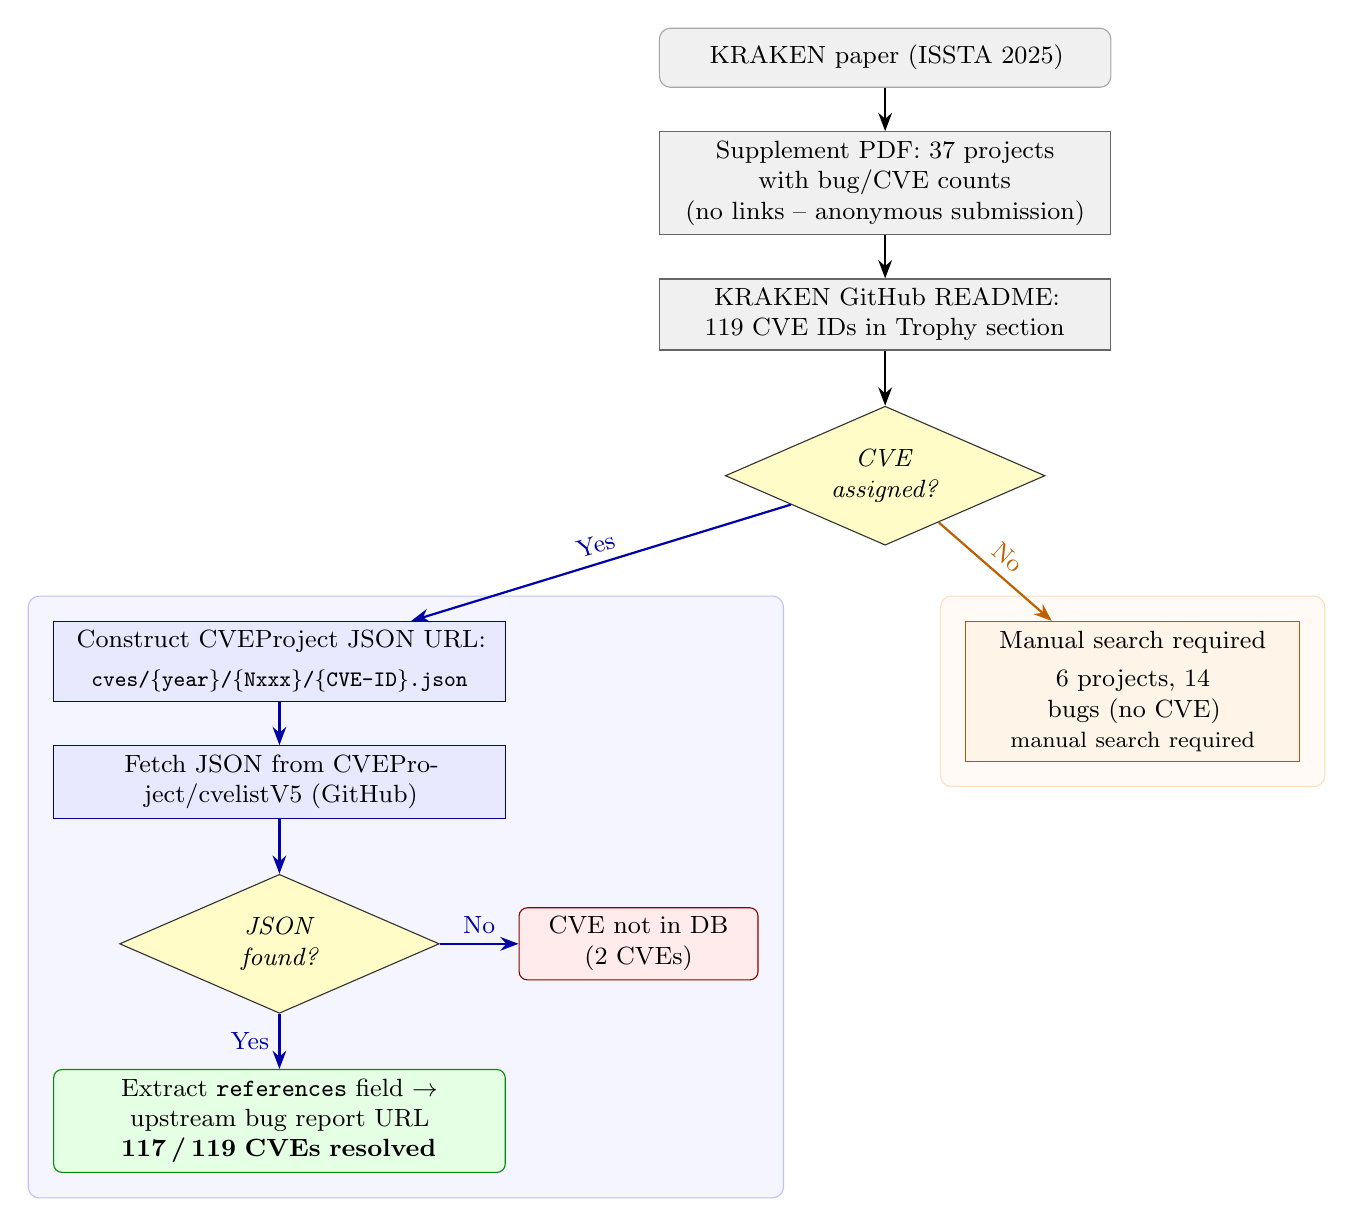
\begin{tikzpicture}[
  node distance = 0.55cm and 1.8cm,
  start/.style   = {rectangle, rounded corners=4pt, draw=gray!70, fill=gray!12,
                    text width=5.5cm, align=center, minimum height=0.75cm, font=\small},
  shared/.style  = {rectangle, draw=black!60, fill=black!6,
                    text width=5.5cm, align=center, minimum height=0.75cm, font=\small},
  cvebox/.style  = {rectangle, draw=blue!60!black, fill=blue!9,
                    text width=5.5cm, align=center, minimum height=0.75cm, font=\small},
  ncvebox/.style = {rectangle, draw=orange!70!black, fill=orange!9,
                    text width=4cm, align=center, minimum height=0.75cm, font=\small},
  decide/.style  = {diamond, aspect=2.3, draw=black!80, fill=yellow!22,
                    text width=2.3cm, align=center, font=\small\itshape, inner sep=1pt},
  ok/.style      = {rectangle, rounded corners=3pt, draw=green!55!black, fill=green!10,
                    text width=5.5cm, align=center, minimum height=0.75cm, font=\small},
  fail/.style    = {rectangle, rounded corners=3pt, draw=red!55!black, fill=red!8,
                    text width=2.8cm, align=center, minimum height=0.7cm, font=\small},
  arr/.style     = {-Stealth, thick},
  cvearr/.style  = {-Stealth, thick, blue!65!black},
  ncvearr/.style = {-Stealth, thick, orange!75!black},
]

%% ── Shared top chain ──────────────────────────────────────────────
\node[start]  (paper)  {KRAKEN paper (ISSTA 2025)};
\node[shared, below=of paper] (supp)
    {Supplement PDF: 37 projects with bug/CVE counts\\(no links -- anonymous submission)};
\node[shared, below=of supp]  (readme)
    {KRAKEN GitHub README:\\119 CVE IDs in Trophy section};
\node[decide, below=0.7cm of readme] (dec) {CVE\\assigned?};

%% ── CVE path (left branch) ────────────────────────────────────────
\node[cvebox, below left=1.4cm and 3.8cm of dec] (url)
    {Construct CVEProject JSON URL:\\[3pt]
     {\footnotesize\texttt{cves/\{year\}/\{Nxxx\}/\{CVE-ID\}.json}}};
\node[cvebox, below=of url] (fetch)
    {Fetch JSON from CVEProject/cvelistV5 (GitHub)};
\node[decide, below=0.7cm of fetch] (jdec) {JSON\\found?};
\node[ok,     below=0.7cm of jdec] (extract)
    {Extract \texttt{references} field $\rightarrow$ upstream bug report URL\\
     \textbf{117\,/\,119 CVEs resolved}};
\node[fail,   right=1.0cm of jdec] (notfound)
    {CVE not in DB\\(2 CVEs)};

%% ── Non-CVE path (right branch, intentionally incomplete) ─────────
\node[ncvebox, below right=1.4cm and 0cm of dec] (manual)
    {Manual search required\\[3pt]
     {\small 6 projects, 14 bugs (no CVE)}\\
     {\footnotesize manual search required}};

%% ── Arrows ────────────────────────────────────────────────────────
\draw[arr]    (paper)  -- (supp);
\draw[arr]    (supp)   -- (readme);
\draw[arr]    (readme) -- (dec);

\draw[cvearr] (dec)   -- node[above,sloped,font=\small]{Yes} (url);
\draw[cvearr] (url)   -- (fetch);
\draw[cvearr] (fetch) -- (jdec);
\draw[cvearr] (jdec)  -- node[left,  font=\small]{Yes} (extract);
\draw[cvearr] (jdec)  -- node[above, font=\small]{No}  (notfound);

\draw[ncvearr] (dec) -- node[above,sloped,font=\small]{No} (manual);

%% ── Background shading ────────────────────────────────────────────
\begin{scope}[on background layer]
  \node[inner sep=9pt, fill=blue!4, draw=blue!25, rounded corners,
        fit=(url)(fetch)(jdec)(extract)(notfound)] {};
  \node[inner sep=9pt, fill=orange!4, draw=orange!25, rounded corners,
        fit=(manual)] {};
\end{scope}

\end{tikzpicture}
\caption{Search process for locating KRAKEN bug reports.
  \textcolor{blue!55!black}{\textbf{Blue:}} CVE-based path -- 119 CVE IDs traced through
  the CVEProject JSON database; 117 links confirmed, 2 not found.
  \textcolor{orange!70!black}{\textbf{Orange:}} Non-CVE path -- 14 bugs across 6 projects
  with no CVE assignments; requires manual issue tracker search (incomplete).}
\label{fig:flowchart}
\end{figure}

\paragraph{Step 1 --- Supplement PDF.}
The paper's \href{https://github.com/seviezhou/Kraken/blob/main/supplement/supplement-material.pdf}{supplement PDF}
provides a table of all 37 target projects, each with the number of bugs found and the
number of CVEs assigned. It contains no CVE IDs and no links to bug reports, as both were
withheld for anonymity during the review period.

\paragraph{Step 2 --- KRAKEN GitHub README.}
The KRAKEN repository at \url{https://github.com/seviezhou/Kraken} contains a Trophy
section in its \texttt{README.md} that lists all 119 CVE IDs in full. These were extracted
as the complete input set for the CVE-based search path.

\paragraph{Step 3 --- Constructing the CVEProject JSON URL.}
Each CVE ID maps to a JSON record in the \texttt{CVEProject/cvelistV5} GitHub repository.
The path is derived mechanically: the year and the first part of the numeric ID determine
the directory. For example:

\begin{center}
\small\renewcommand{\arraystretch}{1.3}
\begin{tabular}{@{}ll@{}}
\toprule
CVE ID   & \texttt{CVE-2021-39550} \\
Year     & \texttt{2021} \\
Number   & \texttt{39550} $\;\Rightarrow\;$ folder \texttt{39xxx} \\
JSON URL & \href{https://raw.githubusercontent.com/CVEProject/cvelistV5/main/cves/2021/39xxx/CVE-2021-39550.json}{\texttt{.../cves/2021/39xxx/CVE-2021-39550.json}} \\
\midrule
\texttt{references} field & \url{https://github.com/sahaRatul/sela/issues/30} \\
\bottomrule
\end{tabular}
\end{center}

\noindent The \texttt{references} field in the JSON record is the upstream bug report filed
by the authors. This one step resolved \textbf{117 out of 119 CVEs}.

\paragraph{Step 4 --- Direct issue tracker search (non-CVE path).}
Six projects carry bugs but no CVE IDs: \textit{advancecomp}, \textit{asn1c},
\textit{jhead}, \textit{libnsfdb}, \textit{nasm}, and \textit{sox}. Their reports require
a manual keyword search of each project's tracker.

%----------------------------------------------------------------------
\section{Summary by Project}
\label{sec:summary}

Table~\ref{tab:summary} summarises all 37 projects from the paper's supplement, along with
the number of bugs found, CVEs assigned, and the number of confirmed bug report links
located in this search.

\input{generated/table_summary}

\noindent\textbf{Notes:}
\begin{itemize}[nosep]
    \item ffmpeg has 1 CVE but that CVE references 3 separate Trac tickets (\#8845, \#8859, \#8860).
    \item gpac and libredwg each report 9 CVEs; one CVE per project could not be fetched from
          the CVEProject database (\texttt{CVE-2020-23927} and \texttt{CVE-2020-20817} respectively).
    \item 6 projects with 0 CVEs account for 14 bugs with no confirmed links.
\end{itemize}

%----------------------------------------------------------------------
\section{Detailed Bug Report Links}
\label{sec:links}

Table~\ref{tab:cves} lists all 119 CVEs, grouped by project, along with the bug type
inferred from the CVE description, a clickable link to the upstream bug report, and a link
to the source CVE JSON record. Each row corresponds to one unique bug report. Where a single
CVE references multiple upstream tickets (e.g.\ ffmpeg), one row is added per ticket.

\begin{center}
\small\renewcommand{\arraystretch}{1.25}
\begin{tabular}{@{}ll@{}}
\toprule
\textbf{Abbreviation} & \textbf{Meaning} \\
\midrule
Heap OOB       & Heap-based buffer overflow or over-read \\
Stack OOB      & Stack-based buffer overflow or over-read \\
Global OOB     & Global buffer overflow or over-read \\
Null Deref     & Null pointer dereference \\
Use After Free & Use-after-free \\
Double Free    & Double free \\
FPE            & Floating point exception \\
Segfault       & Segmentation fault (type unspecified) \\
Unknown        & Could not be inferred from CVE record \\
N/A            & CVE record not in database \\
\bottomrule
\end{tabular}
\end{center}

\input{generated/table_cves}

%----------------------------------------------------------------------
\section{Observations}

To be completed.

\end{document}